\documentclass{homework}

\usepackage{graphicx}
\usepackage{xspace}


\newcommand{\kat}{Kathará\xspace}
\newcommand{\opn}{OPNsense\xspace}
\newcommand{\vb}{VirtualBox\xspace}

\newcommand{\client}{\textit{client}\xspace}
\newcommand{\dmz}{\textit{DMZ}\xspace}
\newcommand{\ser}{\textit{internal server}\xspace}
\newcommand{\intfw}{\textit{intfw}\xspace}
\newcommand{\mainfw}{\textit{mainfw}\xspace}

\newcommand{\lan}{\textit{LAN}\xspace}
\newcommand{\opt}{\textit{OPT1}\xspace}
\newcommand{\wan}{\textit{WAN}\xspace}


\title{Practical Network Defense - Lab 4}
\author{Alessandro Serpi - 1647244}
\date{22 March 2019}


\begin{document}
    \maketitle
    \tableofcontents
    
    \medskip
    
    
    \section{Introduction}
    The private network of \textit{ACME co.} is composed by four subnetworks living in the shared address space \texttt{100.64.0.0/16}. \dmz is connected directly to the main firewall-router \mainfw and offers services accessible from the external network, while \client and \ser networks are behind a second line of defence (represented by the internal firewall-router \intfw). The latter offers services that may be used only by hosts in the private network, whereas the former does not offer any services.
    
    All hosts are already configured (however, minor adjustment may be made), with the exception of the firewalls, that have yet to be created. 
    
    
    \section{Setup of the infrastructure}
    \subsection{Disabling checksum offload}
    The command \texttt{ethtool -K eth0 tx off} was added to every \texttt{.startup} file. This disables the checksum computation offload to the network card; instead, the hosts rely on the CPU to calculate the packet checksums. It is slower, but creates less problems with \opn.
    In \opn, checksum offload is disabled by default.
    
    \subsection{Enabling recursive DNS queries}
    Recursive DNS queries are not permitted, but this clashes with the fact that client hosts are allowed to retrieve web pages from the internet. Therefore, it has been decided to allow recursive DNS queries adding the clause \texttt{recursion yes;} in \texttt{dns/etc/named.conf}, section \texttt{options}.
    
    It has also decided that hosts in the \dmz and in the \ser networks should not be interested in retrieving IP addresses of external websites. Hence, recursive DNS queries have been allowed only for \client network.
    
    \subsection{Creating and configuring the VMs}
    Create in \vb two virtual machine, one for \mainfw and the other for \intfw, each with its own disk. Download the ISO installer from \opn's \href{https://opnsense.org/download/}{official website} and add it to the virtual machines. \href{https://docs.opnsense.org/manual/install.html}{Install} \opn in both machine, then power them off and remove the ISO.
    Finally, add to \mainfw one NAT network card and two bridge adapters and add to \intfw three bridge adapters.
    
    \subsection{Starting the lab}
    Every time it is necessary to launch the lab, use \texttt{lstart} to initiate \kat and then execute \texttt{start\_vms.sh}.
    The script automatically configures the virtual network cards and powers up the virtual machines. 
    
    \subsection{Configuring the interfaces}
    Power up both virtual machine, login as root and enter interface assignment menu. Use \texttt{em0} as \wan, \texttt{em1} as \opt and \texttt{em2} as \lan.
    
    Enter the IP address configuration menu. In \mainfw, configure \wan to use DHCP, assign \texttt{100.64.254.1/30} to \lan and \texttt{100.64.6.1/24} to \opt; in \intfw, assign address \texttt{100.64.254.2/30} and gateway \texttt{100.64.254.1} to \wan, address \texttt{100.64.2.1/24} to \lan and \texttt{100.64.1.1/24} to \opt.
    
    \subsection{Setting up \opn}
    In \mainfw, enter the shell and execute \texttt{route add -inet 100.64.0.0/16 -link \\ 100.64.254.2}. This is a temporary measure in order to access the web GUI from the host. From now on, all operations will be executed through the GUI, accessible at \url{https://100.64.254.1} for \mainfw and \url{https://100.64.2.1} for \intfw. In \mainfw, add route \texttt{100.64.0.0/16} using gateway \texttt{100.64.254.2}.
    
    Disable outbound NAT in \intfw (unnecessary, as it is an internal firewall) and outbound DNS in both machines (DNS servers are configured statically in each host). In \mainfw, set outbound NAT in manual mode and create a rule for NATting the traffic that leaves the private network.
    
    
    \section{Evaluation of the security policy}
    \subsection{DNS}
    All internal hosts should be able to resolve internal domain names.
    Since devices in the \textit{client} network are the only ones that can access external web services, no other host should be able to resolve external domains,
    
    \subsection{FTP}
    All internal hosts should be able to connect to the internal FTP server, while only devices in \textit{client} network should be able to connect to external ones.
    External hosts should be able to connect to the internal FTP server.
    
    \subsection{HTTP/HTTPS}
    All internal hosts should be able to connect to the internal web server, while only devices in \textit{client} network should be able to connect to external websites and to the firewall-router administration pages.
    External hosts should be able to connect to the internal web server.
    
    \subsection{SSH}
    Hosts in \textit{client} network should be able to use the SSH protocol in the internal network.
    No other use is authorised.
    
    \subsection{Syslog}
    Internal hosts should be able to send logging messages to the syslog server.
    No other use is authorised.
    
    
    \section{Policy implementation in \opn}
    There are two types of rules in \opn: floating and interface.
    Floating rules apply to all packets and (with \texttt{quick} option enabled) have the highest precedence, while interface rules apply only to packets arriving in a specific interface.
    Unless otherwise stated, enabling a rule automatically creates a reply-to inverse rule that allows reply packets.
    Since the network topology is quite simple, only interface rules have been used.
    
    \subsection{Default policy}
    Packets not matched by any rule are logged and blocked.
    Since \opn adopts the opposite default policy for LAN interfaces, the chosen behaviour has been manually enforced everywhere.
    
    \subsection{Address spoofing}
    To avoid IP address spoofing, firewalls reject packets coming from IP addresses not belonging to the subnet the receiving interface is connected to.
    
    \subsection{Aliases}
    To each relevant address (or address range) has been assigned an alias.
    When formulating firewall or port forwarding rules, we can use the alias instead of the correspondent address, increasing readability and decreasing the possibility of errors.
    
    \subsection{Packets arriving to \mainfw from\dots}
    \subsubsection{\dots \dmz}
    \begin{figure}[H]
        \centering
        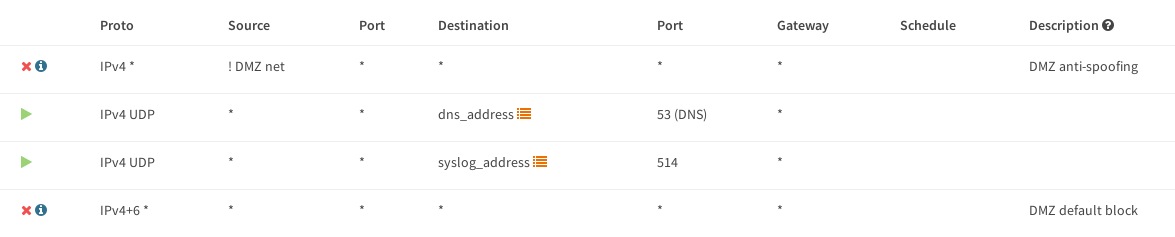
\includegraphics[width=\linewidth]{images/mainfw-DMZ}
        \label{fig:mainfw-dmz}
    \end{figure}
    
    \subsubsection{\dots outside}
    \begin{figure}[H]
        \centering
        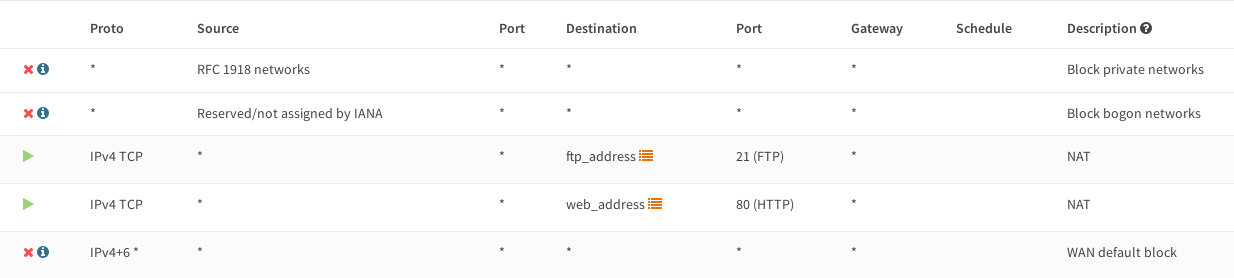
\includegraphics[width=\linewidth]{images/mainfw-wan}
        \label{fig:mainfw-wan}
    \end{figure}
    
    \begin{figure}[H]
        \centering
        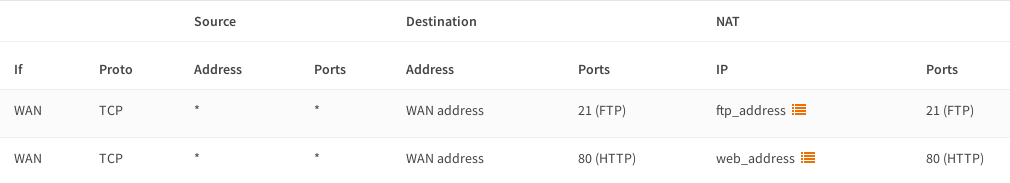
\includegraphics[width=\linewidth]{images/mainfw-portforwarding}
        \label{fig:mainfw-portforwarding}
    \end{figure}
    Since the FTP and the web servers provide public services but have no public IP address, it is necessary to enable port forwarding.
    
    \subsubsection{\dots \intfw}
    \begin{figure}[H]
        \centering
        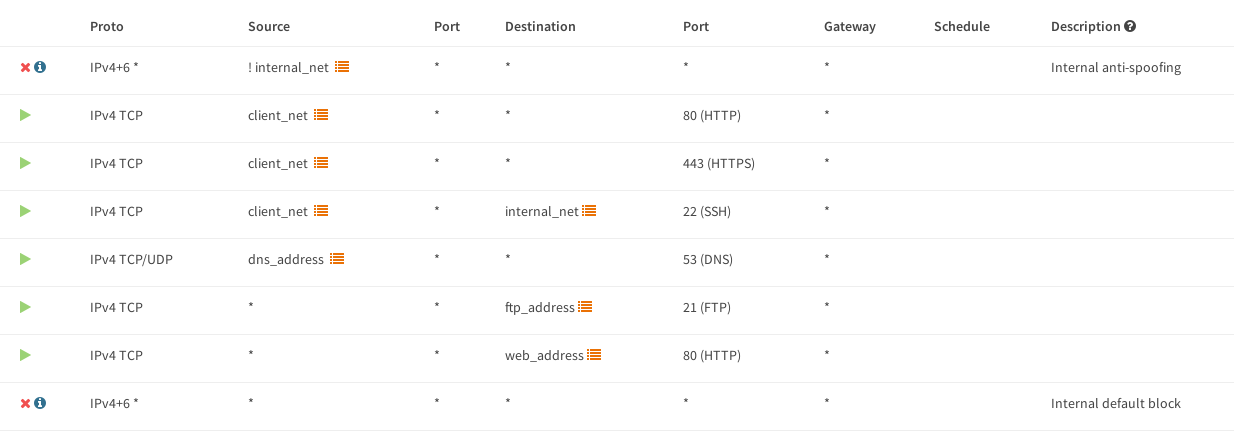
\includegraphics[width=\linewidth]{images/mainfw-internal}
        \label{fig:mainfw-internal}
    \end{figure}
    An attacker that has compromised \intfw (or the link between the firewalls) is able to spoof address in \dmz.
    However, this small risk is greatly surpassed by the additional flexibility: it is possible to add a new low-privilege internal subnet without modifying firewall rules.
    
    \subsection{Packets arriving to \intfw from \dots}
    \subsubsection{\dots \mainfw}
    \begin{figure}[H]
        \centering
        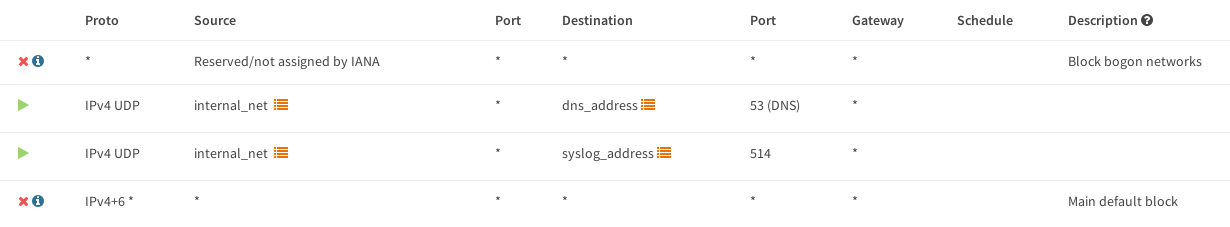
\includegraphics[width=\linewidth]{images/intfw-main}
        \label{fig:intfw-main}
    \end{figure}
    Similarly to the previous section, an attacker that has compromised \mainfw (or the link between the firewalls) is able to spoof addresses in \client or \ser networks.
    
    \subsubsection{\dots the \client network}
    \begin{figure}[H]
        \centering
        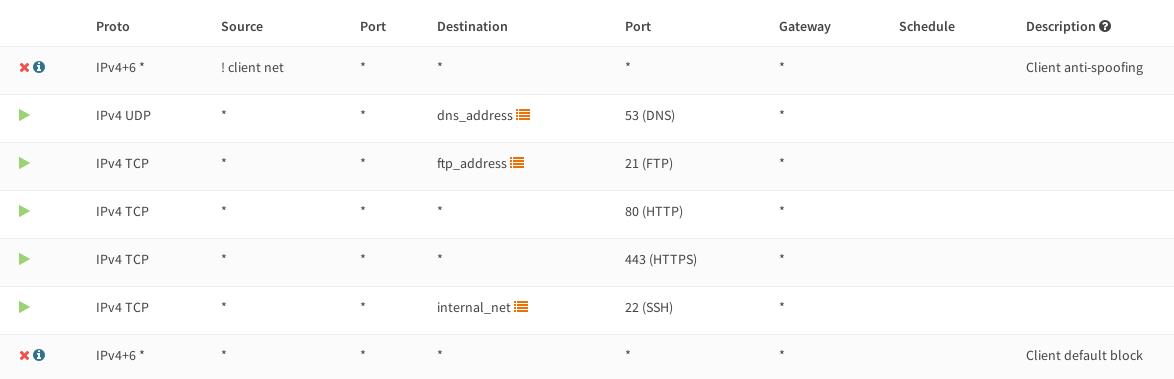
\includegraphics[width=\linewidth]{images/intfw-client}
        \label{fig:intfw-client}
    \end{figure}
    
    \subsubsection{\dots the \ser network}
    \begin{figure}[H]
        \centering
        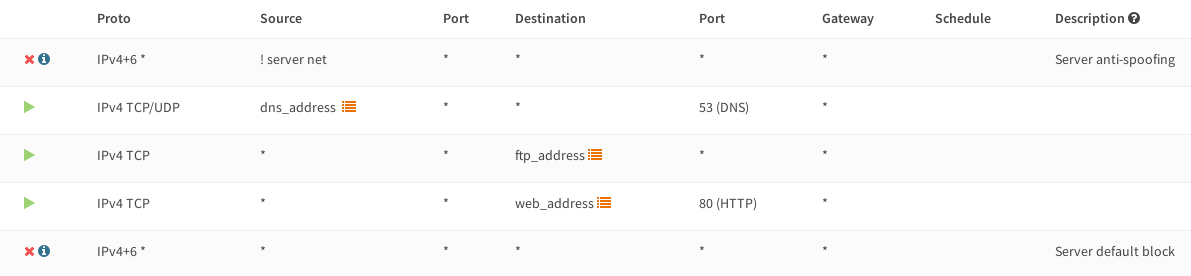
\includegraphics[width=\linewidth]{images/intfw-server}
        \label{fig:intfw-server}
    \end{figure}
    
    
    \section{Test of the configuration}
    In the root directory of each \kat  host there is an executable script \texttt{$\langle$host$\rangle$.test} that checks the firewall and DNS functionality.
    The return code is a 4-bit flag:
    \begin{itemize}
        \item \texttt{0001}: error on DNS resolution of internal hosts
        \item \texttt{0010}: error on DNS resolution of external hosts
        \item \texttt{0100}: error on internal web connectivity
        \item \texttt{1000}: error on external web connectivity.
    \end{itemize}
    
    Given that \textit{expect} is not installed and both \textit{ftp} and \textit{ssh} clients can not be reliably used with simple bash scripts, testing the corresponding protocols must be done manually, checking the connectivity for each host.
    
    
    \section{Final remarks}
    When checksum offload is activated, all packets passing through the firewall get corrupted. Disabling it on the host's virtual interfaces produce no effects, it must be done from the \kat hosts.
    
    In theory, outbound NAT should be disabled in \mainfw, as \vb already takes care of translating the IP addresses. In practice, disabling it conflicts with the configuration script.
\end{document}
